\chapter{CIVITA Geometry Library Catalog}
\label{app:geometry-library}


\section{Introduction and Conventions}
\label{sec:geometry-definitions}

This catalog presents the standardized geometry definitions included in the CIVITA Geometry Library. Each geometry type is identified by a unique global identifier and version number and is characterized by a reference figure, a local right-handed Cartesian coordinate system, a set of independent geometric parameters, and, where applicable, derived parameters and geometric constraints.

The definitions establish the geometric meaning, units, and admissible ranges of the parameters independently of their application to specific experimental specimens or computational models. Individual geometry instances are obtained by assigning numerical values to the independent parameters in accordance with the corresponding definition. Unless otherwise specified, geometric dimensions are expressed in millimeters.

The following subsections document the seven geometry types currently available in the library, ordered by their global identifiers. The authoritative machine-readable specifications are maintained in the CIVITA common specifications repository (\texttt{civita-schema}). In case of discrepancies, the corresponding version of the authoritative JSON definition governs the interpretation of the geometry.




%============================================================
\subsection{\texttt{prism}}
\label{subsec:geometry_prism}
%============================================================

\noindent
\textbf{Geometry ID:} \texttt{GLOB-GEO0001}
\qquad
\textbf{Version:} \texttt{1.0.0}

\begin{figure}[htbp]
    \centering
    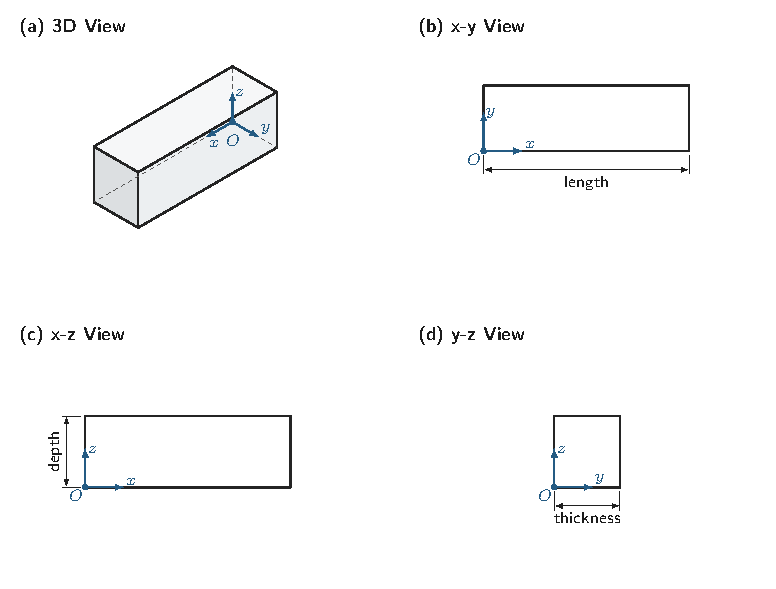
\includegraphics[width=0.7\linewidth]
    {./figs/geometries/prism.pdf}
    \caption{Standardized parametrization and local
    coordinate system of the prism geometry.}
    \label{fig:prism}
\end{figure}

The \texttt{prism} geometry represents a rectangular
prismatic specimen. As illustrated in
Fig.~\ref{fig:prism}, the local coordinate system
is defined by the right-handed Cartesian axes
$x$, $y$, and $z$, with the origin located at
the reference corner indicated in the figure.

The $x$ axis represents the longitudinal direction,
the $y$ axis the transverse thickness direction,
and the $z$ axis the specimen depth direction.

\paragraph{Independent parameters.}

The geometry is defined by three required parameters,
all expressed in millimeters:

\begin{itemize}
    \item \texttt{length}: specimen dimension along
    the local $x$ axis;

    \item \texttt{thickness}: specimen dimension
    along the local $y$ axis;

    \item \texttt{depth}: specimen dimension along
    the local $z$ axis.
\end{itemize}

\paragraph{Geometric constraints.}

All three parameters must be strictly positive.




%============================================================
\subsection{\texttt{cube}}
\label{subsec:geometry_cube}
%============================================================

\noindent
\textbf{Geometry ID:} \texttt{GLOB-GEO0002}
\qquad
\textbf{Version:} \texttt{1.0.0}

\begin{figure}[htbp]
    \centering
    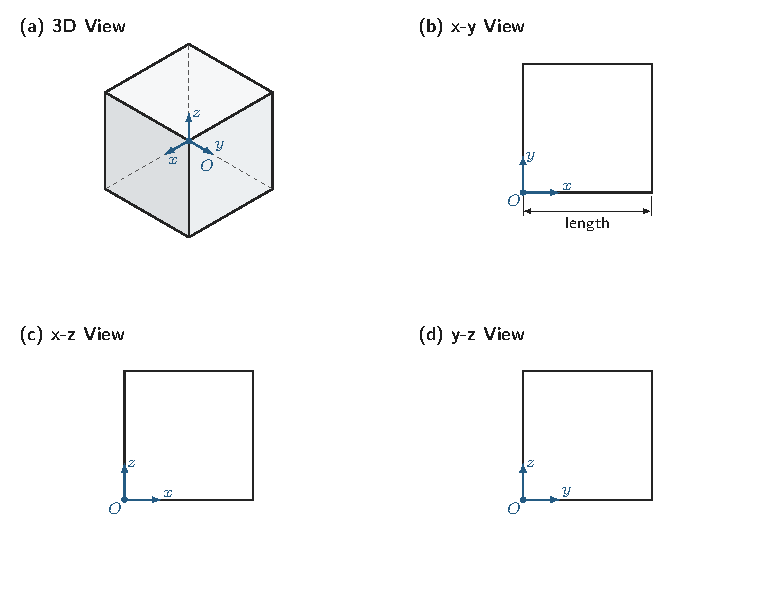
\includegraphics[width=0.7\linewidth]
    {./figs/geometries/cube.pdf}
    \caption{Standardized parametrization and local
    coordinate system of the cube geometry.}
    \label{fig:cube}
\end{figure}

The \texttt{cube} geometry represents a cubic
specimen with equal dimensions along three mutually
orthogonal directions. As illustrated in
Fig.~\ref{fig:cube}, the local coordinate system
is defined by the right-handed Cartesian axes
$x$, $y$, and $z$, with the origin located at
the reference corner indicated in the figure.

The three coordinate axes are aligned with the
edges of the cube.

\paragraph{Independent parameters.}

The geometry is defined by one required parameter,
expressed in millimeters:

\begin{itemize}
    \item \texttt{length}: cube edge length,
    corresponding to the dimensions along
    the local $x$, $y$, and $z$ directions.
\end{itemize}

\paragraph{Geometric constraints.}

The parameter \texttt{length} must be strictly
positive.




%============================================================
\subsection{\texttt{cylinder}}
\label{subsec:geometry_cylinder}
%============================================================

\noindent
\textbf{Geometry ID:} \texttt{GLOB-GEO0003}
\qquad
\textbf{Version:} \texttt{1.0.0}

\begin{figure}[htbp]
    \centering
    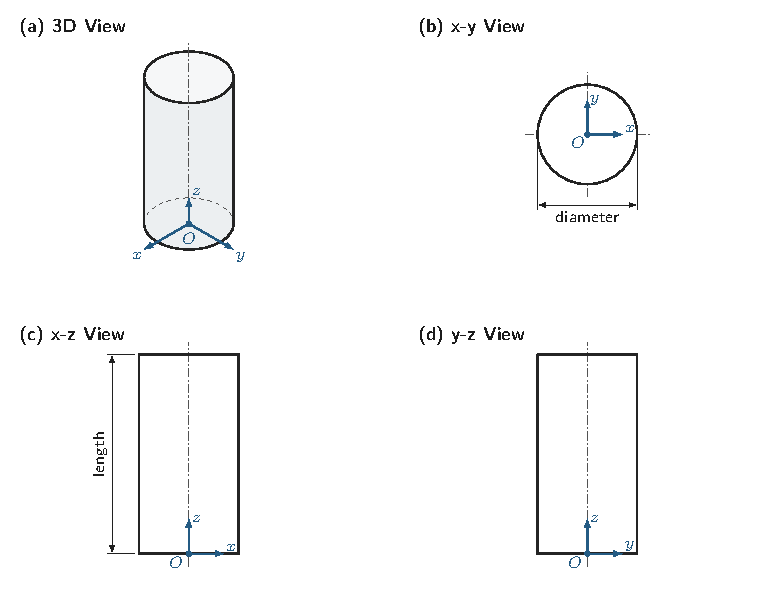
\includegraphics[width=0.7\linewidth]
    {./figs/geometries/cylinder.pdf}
    \caption{Standardized parametrization and local
    coordinate system of the cylinder geometry.}
    \label{fig:cylinder}
\end{figure}

The \texttt{cylinder} geometry represents a right
circular cylindrical specimen. As illustrated in
Fig.~\ref{fig:cylinder}, the local coordinate
system is defined by the right-handed Cartesian
axes $x$, $y$, and $z$.

The origin $O$ is located at the center of the
reference circular end face, corresponding to
$z=0$. The $z$ axis coincides with the longitudinal
axis of the cylinder and extends toward the opposite
end face at $z=\texttt{length}$. The $x$ and $y$
axes define the transverse plane of the circular
cross section.

\paragraph{Independent parameters.}

The geometry is defined by two required parameters,
both expressed in millimeters:

\begin{itemize}
    \item \texttt{length}: longitudinal specimen
    dimension along the local $z$ axis;

    \item \texttt{diameter}: diameter of the
    circular cross section in the local
    $x$--$y$ plane.
\end{itemize}

\paragraph{Geometric constraints.}

Both parameters must be strictly positive.


\subsection{\texttt{notched\_prism}}
\label{subsec:geometry_notched_prism}

\noindent
\textbf{Geometry ID:} \texttt{GLOB-GEO0004}
\qquad
\textbf{Version:} \texttt{1.0.0}

\begin{figure}[htbp]
    \centering
    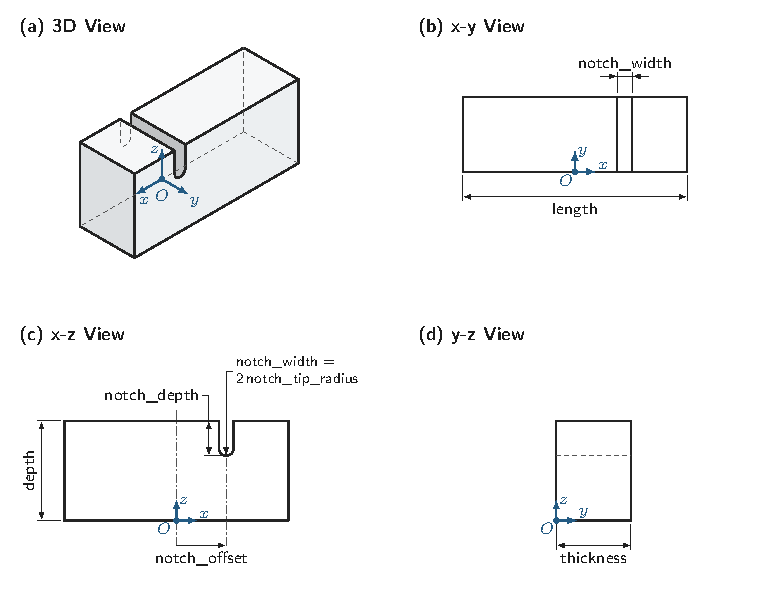
\includegraphics[width=0.65\linewidth]
    {./figs/geometries/notched_prism.pdf}
    \caption{Standardized parametrization and local
    coordinate system of the notched prism geometry.}
    \label{fig:notched_prism}
\end{figure}

The \texttt{notched\_prism} geometry represents a rectangular
prismatic specimen containing a notch with parallel sides
and a semicircular tip. As illustrated in
Fig.~\ref{fig:notched_prism}, the local coordinate system
is defined by the right-handed Cartesian axes $x$, $y$,
and $z$. The origin $O$ is located at longitudinal midspan
on the intersection of the reference face $y=0$ and
the face $z=0$.

The $x$ axis represents the longitudinal direction,
the $y$ axis the transverse thickness direction,
and the $z$ axis the specimen depth direction.
Relative to the origin, the specimen occupies the region
$-\texttt{length}/2 \leq x \leq \texttt{length}/2$,
$0 \leq y \leq \texttt{thickness}$, and
$0 \leq z \leq \texttt{depth}$.

\paragraph{Independent parameters.}

The geometry is defined by six required parameters,
all expressed in millimeters:

\begin{itemize}
    \item \texttt{length}: specimen dimension along
    the local $x$ axis;

    \item \texttt{thickness}: specimen dimension along
    the local $y$ axis;

    \item \texttt{depth}: specimen dimension along
    the local $z$ axis;

    \item \texttt{notch\_offset}: signed $x$ coordinate
    of the notch centerline relative to specimen
    midspan. A value of zero corresponds to a
    centered notch;

    \item \texttt{notch\_depth}: positive distance
    from the notched face to the deepest point
    of the semicircular notch tip, measured
    along the local $z$ direction;

    \item \texttt{notch\_width}: opening width
    of the notch.
\end{itemize}

\paragraph{Derived parameters.}

The notch terminates in a semicircular tip whose
radius is determined by the notch opening width:

\begin{equation}
    \texttt{notch\_tip\_radius}
    = \frac{\texttt{notch\_width}}{2}.
\end{equation}

Consequently, \texttt{notch\_tip\_radius} is a
derived quantity and is not an independent input
parameter.

\paragraph{Geometric constraints.}

All dimensions must be strictly positive, with
the exception of \texttt{notch\_offset}, which
may be positive, negative, or zero.

The notch geometry must additionally satisfy

\begin{align}
    \texttt{notch\_depth}
    &> \frac{\texttt{notch\_width}}{2},
    \\
    \texttt{notch\_depth}
    &< \texttt{depth},
    \\
    \texttt{notch\_offset}
    + \frac{\texttt{notch\_width}}{2}
    &< \frac{\texttt{length}}{2},
    \\
    \frac{\texttt{notch\_width}}{2}
    - \texttt{notch\_offset}
    &< \frac{\texttt{length}}{2}.
\end{align}

The first condition ensures that the notch contains
a straight-sided segment preceding its semicircular
termination. The second prevents the notch from
penetrating the full specimen depth, while the
remaining conditions ensure that the notch remains
within the longitudinal boundaries of the specimen.



%============================================================
\subsection{\texttt{dogbone}}
\label{subsec:geometry_dogbone}
%============================================================

\noindent
\textbf{Geometry ID:} \texttt{GLOB-GEO0005}
\qquad
\textbf{Version:} \texttt{1.0.0}

\begin{figure}[htbp]
    \centering
    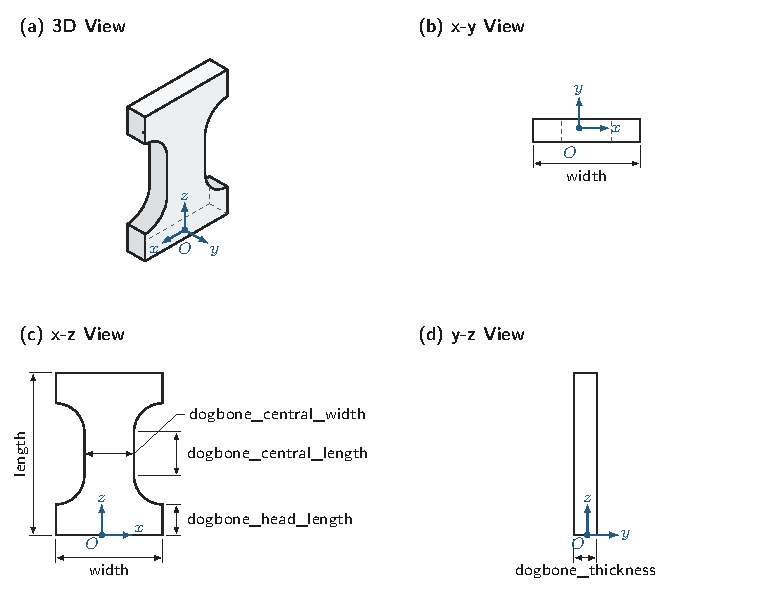
\includegraphics[width=0.65\linewidth]
    {./figs/geometries/dogbone.pdf}
    \caption{Standardized parametrization and local
    coordinate system of the dogbone geometry.}
    \label{fig:dogbone}
\end{figure}

The \texttt{dogbone} geometry represents a specimen
consisting of two identical enlarged heads connected
to a reduced central region through two identical
transition regions.

As illustrated in Fig.~\ref{fig:dogbone}, the
local coordinate system is defined by the
right-handed Cartesian axes $x$, $y$, and $z$,
with the origin located at the reference point
indicated in the figure.

The $z$ axis represents the longitudinal direction,
the $x$ axis the specimen width direction,
and the $y$ axis the thickness direction.

\paragraph{Independent parameters.}

The geometry is defined by six required dimensional
parameters, expressed in millimeters, and one
optional categorical parameter:

\begin{itemize}
    \item \texttt{length}: overall specimen length
    along the local $z$ axis;

    \item \texttt{width}: maximum specimen width,
    measured across the enlarged heads along
    the local $x$ axis;

    \item \texttt{dogbone\_central\_length}:
    longitudinal length of the reduced central
    region;

    \item \texttt{dogbone\_central\_width}:
    width of the reduced central region;

    \item \texttt{dogbone\_head\_length}:
    longitudinal length of each enlarged head;

    \item \texttt{dogbone\_thickness}:
    specimen thickness along the local $y$ axis;

    \item \texttt{transition\_type}:
    optional categorical parameter defining
    the shape of the transition regions.
    Permitted values are
    \texttt{linear\_transition} and
    \texttt{curved\_transition}.
    The default is \texttt{curved\_transition}.
\end{itemize}

The transition type specifies whether the lateral
boundaries connecting the enlarged heads to the
reduced central region are linear or curved.
For curved transitions, the precise curvature
is not prescribed by the current parametrization.

\paragraph{Derived parameters.}

The longitudinal length of each transition region
is determined by

\begin{equation}
\begin{aligned}
\texttt{dogbone\_transition\_length}
= \frac{1}{2}\bigl(
&\texttt{length}
-2\,\texttt{dogbone\_head\_length}\\
&-\texttt{dogbone\_central\_length}
\bigr).
\end{aligned}
\end{equation}

The lateral width reduction on each side of the
specimen is given by

\begin{equation}
\begin{aligned}
\texttt{dogbone\_transition\_width}
=\frac{1}{2}\bigl(
&\texttt{width}\\
&-\texttt{dogbone\_central\_width}
\bigr).
\end{aligned}
\end{equation}

These quantities are derived from the independent
parameters and are not specified separately.

\paragraph{Geometric constraints.}

All required dimensional parameters must be
strictly positive. In addition, the geometry
must satisfy

\begin{align}
\texttt{length}
&>
2\,\texttt{dogbone\_head\_length}
+\texttt{dogbone\_central\_length},
\\
\texttt{width}
&>
\texttt{dogbone\_central\_width}.
\end{align}

These conditions ensure strictly positive
transition lengths and lateral width reductions.



%============================================================
\subsection{\texttt{ell\_shape}}
\label{subsec:geometry_ell_shape}
%============================================================

\noindent
\textbf{Geometry ID:} \texttt{GLOB-GEO0006}
\qquad
\textbf{Version:} \texttt{1.0.0}

\begin{figure}[htbp]
    \centering
    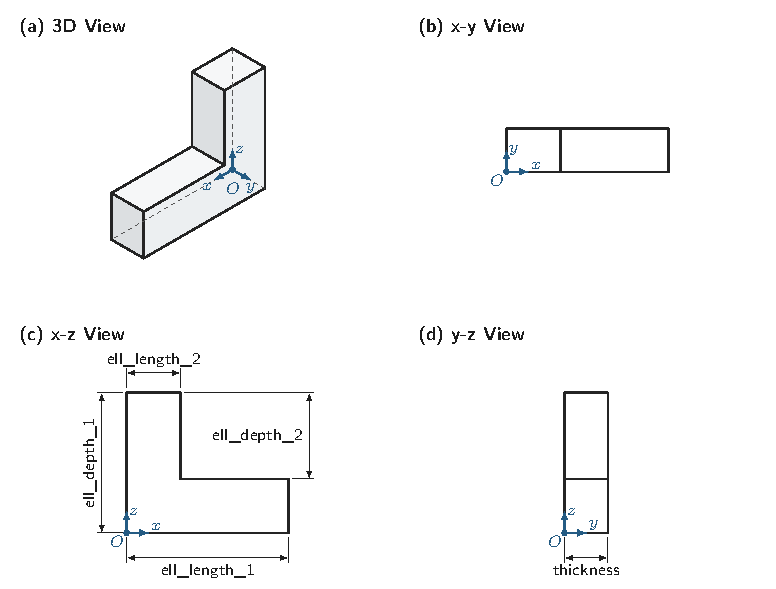
\includegraphics[width=0.65\linewidth]
    {./figs/geometries/ell_shape.pdf}
    \caption{Standardized parametrization and local
    coordinate system of the L-shaped geometry.}
    \label{fig:ell_shape}
\end{figure}

The \texttt{ell\_shape} geometry represents an
L-shaped specimen formed by two orthogonal legs
with uniform thickness.

As illustrated in Fig.~\ref{fig:ell_shape},
the local coordinate system is defined by
the right-handed Cartesian axes $x$, $y$,
and $z$. The origin $O$ is located at the
exterior corner of the L-shaped profile on
the reference face $y=0$, corresponding to
$x=0$ and $z=0$.

The positive $x$ and $z$ directions extend
from the origin into the specimen along
its overall length and depth, respectively.
The $y$ axis represents the thickness direction.

The L-shaped profile lies in the local
$x$--$z$ plane and is extruded along the
positive $y$ direction.

\paragraph{Independent parameters.}

The geometry is defined by five required
parameters, all expressed in millimeters:

\begin{itemize}
    \item \texttt{thickness}: uniform specimen
    thickness along the local $y$ axis;

    \item \texttt{ell\_length\_1}: overall
    specimen dimension along the local $x$ axis;

    \item \texttt{ell\_depth\_1}: overall
    specimen dimension along the local $z$ axis;

    \item \texttt{ell\_length\_2}: width along
    the local $x$ direction of the leg extending
    through the full specimen depth;

    \item \texttt{ell\_depth\_2}: distance along
    the local $z$ direction from the reentrant
    corner to the end of the full-depth leg.
\end{itemize}

The reentrant corner of the L-shaped profile
is located at

\begin{equation}
\begin{aligned}
x &= \texttt{ell\_length\_2},\\
z &= \texttt{ell\_depth\_1}
     -\texttt{ell\_depth\_2}.
\end{aligned}
\end{equation}

\paragraph{Geometric constraints.}

All five parameters must be strictly positive.
The dimensions must additionally satisfy

\begin{align}
\texttt{ell\_length\_2}
&< \texttt{ell\_length\_1},
\\
\texttt{ell\_depth\_2}
&< \texttt{ell\_depth\_1}.
\end{align}

These conditions ensure that both orthogonal
legs have positive dimensions and that
the L-shaped profile contains a well-defined
reentrant corner.



%============================================================
\subsection{\texttt{notched\_cylinder}}
\label{subsec:geometry_notched_cylinder}
%============================================================

\noindent
\textbf{Geometry ID:} \texttt{GLOB-GEO0007}
\qquad
\textbf{Version:} \texttt{1.0.0}

\begin{figure}[htbp]
    \centering
    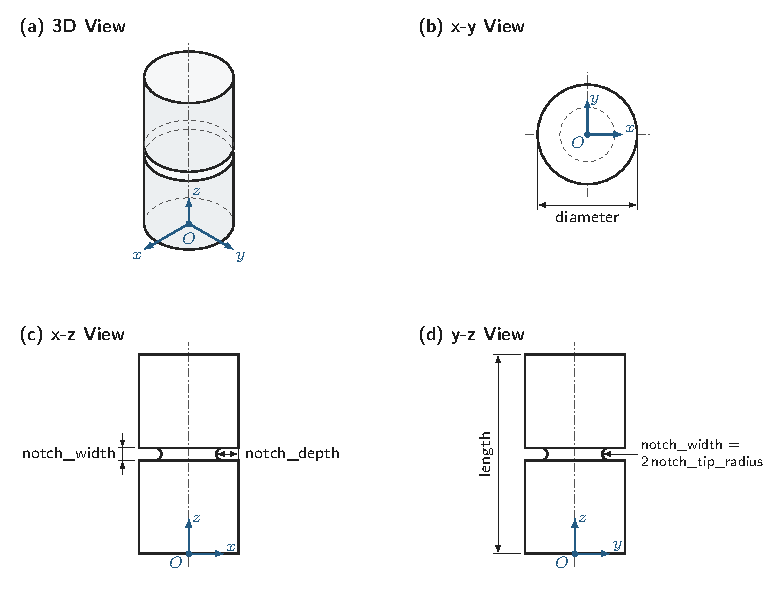
\includegraphics[width=0.65\linewidth]
    {./figs/geometries/notched_cylinder.pdf}
    \caption{Standardized parametrization and local
    coordinate system of the notched cylinder geometry.}
    \label{fig:notched_cylinder}
\end{figure}

The \texttt{notched\_cylinder} geometry represents
a right circular cylindrical specimen containing
an axisymmetric circumferential notch centered
at longitudinal midspan.

As illustrated in Fig.~\ref{fig:notched_cylinder},
the local coordinate system is defined by
the right-handed Cartesian axes $x$, $y$,
and $z$. The origin $O$ is located at
the center of the reference circular end face,
corresponding to $z=0$.

The $z$ axis coincides with the longitudinal
axis of the cylinder, while the $x$ and $y$
axes define the transverse plane.

The circumferential notch is centered at

\begin{equation}
z=\frac{\texttt{length}}{2}.
\end{equation}

In an axial section, the notch has parallel
sides terminating in a semicircular tip.

\paragraph{Independent parameters.}

The geometry is defined by four required
parameters, all expressed in millimeters:

\begin{itemize}
    \item \texttt{length}: cylinder length
    measured along the local $z$ axis;

    \item \texttt{diameter}: outer cylinder
    diameter measured in the local
    $x$--$y$ plane;

    \item \texttt{notch\_depth}: total radial
    penetration measured inward from the
    original cylindrical surface to the
    deepest point of the semicircular tip;

    \item \texttt{notch\_width}: axial opening
    width of the circumferential notch,
    measured along the local $z$ axis.
\end{itemize}

\paragraph{Derived parameters.}

The notch terminates in a semicircular tip
whose radius is determined by

\begin{equation}
\texttt{notch\_tip\_radius}
=\frac{\texttt{notch\_width}}{2}.
\end{equation}

The radius is therefore a derived quantity
and is not an independent input parameter.

\paragraph{Geometric constraints.}

All independent parameters must be strictly
positive. The notch geometry must additionally
satisfy

\begin{align}
\texttt{notch\_depth}
&< \frac{\texttt{diameter}}{2},
\\
\texttt{notch\_width}
&< \texttt{length},
\\
\texttt{notch\_depth}
&> \frac{\texttt{notch\_width}}{2}.
\end{align}

The first condition ensures a strictly positive
remaining radius at the notch root. The second
ensures that the notch remains within the
longitudinal extent of the cylinder. The third
requires a strictly positive straight-sided
radial portion preceding the semicircular tip.


